\documentclass{beamer}

\usetheme{CambridgeUS}

\usepackage{amsmath}
\usepackage{adjustbox}
\usepackage{amsmath}
\usepackage{amssymb}
\usepackage{relsize}
\usepackage{graphicx}
\usepackage{verbatim}
\usepackage{hyperref}
\usepackage{relsize}
\usepackage{amsthm}

\usepackage{pgffor}%
\usepackage{geometry}
\usepackage{pdflscape}

\usepackage[utf8]{inputenc}
\usepackage[english]{babel}


\newtheorem{proposition}[theorem]{Proposition}
\newtheorem{assumption}[theorem]{Assumption}

\title{Impacts of Taxes on Firm Location}
\author{Kevin D. Duncan}
\institute{Iowa State University}
\date{MEA, Apr 1st, 2016}

\begin{document}

\begin{frame}
\title{Impacts of Taxes on Firm Entry Rates along State Borders}
\author{Kevin D. Duncan}
\institute{Iowa State University}
\date{Midwest Econ Associaton \\ April 1st, 2016}
\maketitle
\end{frame}

\begin{frame}
\section{Introduction \& Motivation}
\frametitle{Introduction \& Motivation}
\begin{itemize}
\item Do changes in tax and regulatory policy impact firm entry?
\item Do firms have preferences for government provided amenities?
\item Changing tax rates are a major policy lever for state officials looking to impact the economy, or raise tax revenue. Understanding these impacts are invaluable, especially for states that face balanced budget requirements, such that understanding the estimated dynamic effects of these changes is very important.
\begin{itemize}
\item Two examples are tax cuts done by Gov. Brownback of Kansas, who expected large growth returns to tax cuts, but revenue hasn't recouped itself fast enough, and now requires massive restructuring of the budget. Alternatively, Sen. Bernie Sanders' requires raising new tax revenue to fund a variety of plans, but might impose large costs on the economy.
\end{itemize}
\end{itemize}
\end{frame}


\begin{frame}
\section{Addition to the Literature}
\frametitle{Addition to the Literature}
Our motivation
\begin{itemize}
\item We add to the literature by using the longest array of top marginal tax rates used to date and buld on top of current regression discontinuity approaches.
\begin{itemize}
\item This accounts for joint tax policy changes that policy makers may do to shif tax burdens around, as well as changes in tax policy aimed at affecting state revenue
\end{itemize}
\item  Many papers do not include marginal tax rates, where theory indicates firms and individuals respond to marginal rates when making entry decisions.
\begin{itemize}
\item Economic theory shows that marginal rates enter into the first order conditions of firms and individuals looking on optimal location choice.
\end{itemize}
\end{itemize}
\end{frame}

\begin{frame}
\section{Literature Review}
\frametitle{Literature Review}
\begin{itemize}
\item Early papers used conditional logit models to estimate firm entry across all counties. Often found positive relationship between taxes and firm entry rates. Carlton (1979, 1983), Schmenner (1975, 1982).
\item Modern papers have started to use border discontinuity effects to look at impacts of policies on firm entry rates. Chirinko and Wilson (2008), Rathelot and Sillard (2008), Duranton et al (2011), Rohlin, Rosenthal, and Ross (2014)
\item Across all papers there has been a variety of taxes used. 
\begin{itemize}
\item  Carlton (1983) used weighted top marginal tax corporate and income tax rates, and a second term for property tax rates. 
\item Schmenner (1987) uses state and local property tax revenues per dollar of personal income. 
\item Helms (1985) used a budget constraint to estimate the impacts of rising tax revenue on explanatory variables.
\end{itemize}
\end{itemize}
\end{frame}


\begin{frame}
\section{Data}
\frametitle{Data}
\begin{itemize}
\item Total number of firm start ups in every continental US county
\item Seven different state top marginal tax rates
\begin{itemize}
\item property, income, capital gains, sales, corporate, workers compensation, unemployment insurance
\end{itemize}
\item Log state expenditures per capita on education, highways, and welfare
\item Scaled county geographic amenities: Pct of area that is water, average humidity in july, average temperature in january, topology score
\item Additional (state level) Controls: County level real fuel prices, pct with high school  education, population density, pct unionized, pct manufacturing
\end{itemize}
\end{frame}

\begin{frame}
\subsection{Regression Discontinuity Model}
\frametitle{Regression Discontinuity Model pt I}
\begin{itemize}
\item Naive estimation of firm entry decisions over all available counties doesn't account for policy changes that occur with respect to current economic behavior. High performing states may increase taxes to raise revenue, and low performing states may cut taxes to increase growth rates. This upwards biases traditional estimates. 
\item By assuming that state policy does not respond to shocks along state borders, we take the difference in matched county pairs along state pair borders. This controlls for shared macroeconomic shocks that occur on both sides of the border, as well as local economic shocks that are continuous around the border.
\end{itemize}
\end{frame}

\begin{frame}
\frametitle{Regression Discontinuity Model pt II}
\begin{figure}[h]\label{rb}
    \centering
    \textbf{Example of Border Matching}
    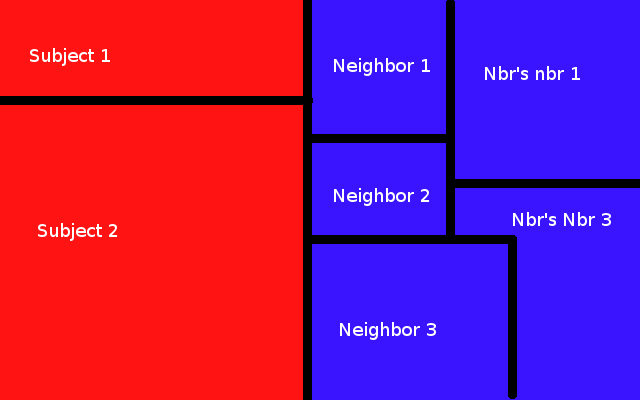
\includegraphics[scale = 0.35]{../../analysis/output/borders_temp.png}
    \caption{Red rectangles are subject counties, and blue are neighbor counties. In this example Subject 1 would be only matched to Neighbor 1, while "Subject 2" would be paired with Neighbor 1-3. Similarly, when we broaden the bandwidth, Subject 1 would be matched with Nbr's Nbr 1, whle Subject 2 would be paired with Nbr's Nbr 1 and 2}
\end{figure}
\end{frame}

\begin{frame}
\frametitle{Regression Discontinuity Model pt III}
\begin{itemize}
\item Assume for counties, we have local entry behavior defined by,
$$ ln(n_{ijt}) = \gamma_{j}+X_{i,j,t-1}\beta + e_{ijt}$$
\item $n_{ijt}$ is the number of firms that entery in a county $i$ in state $j$ in time period $t$, $\gamma$ is a constant, $X_{i,j,t-1}$ is a set of covariates with coefficient $\beta$, and $e_{ijt}$ is a mean zero error term.
\item Now define the variables
 $$\ddot{ln(n_{i,g,t})} = ln(n_{sub,A,t})-ln(n_{nbr,B,t})$$
 $$\ddot x_{g,t-1} = x_{A,t-1}-x_{B,t-1}$$
 $$\ddot \epsilon_{i,g,t} = \epsilon_{sub,A,t}-\epsilon_{nbr,B,t}$$
Where $i$ now indexes matched counties on either side of a state border. This leads to the differenced equation
\begin{equation}\label{fe}
\ddot \ln(n_{i,g,t}) = \gamma_{A}-\gamma_{B}+\ddot X_{g,t-1}\beta + \ddot \epsilon_{i,g,t}
\end{equation}
\end{itemize}
\end{frame}



\begin{frame}
\frametitle{RD Results}
% Table created by stargazer v.5.2 by Marek Hlavac, Harvard University. E-mail: hlavac at fas.harvard.edu
% Date and time: Tue, Oct 13, 2015 - 02:44:06 PM
\begin{table}[!htbp] \centering 
  \caption{Regression Discontinuity Models for  Total Firm Births} 
  \label{--rd} 
  \tiny
  {\tiny\renewcommand{\arraystretch}{}
\resizebox{!}{.35\paperheight}{%
\begin{tabular}{@{\extracolsep{5pt}}lcccc} 
\\[-1.8ex]\hline 
\hline \\[-1.8ex] 
 & \multicolumn{4}{c}{\textit{Dependent variable:}} \\ 
\cline{2-5} 
\\[-1.8ex] & \multicolumn{3}{c}{births ratio} & births\_ratio \\ 
 & OLS & OLS & OLS & FE \\ 
\\[-1.8ex] & (1) & (2) & (3) & (4)\\ 
\hline \\[-1.8ex] 
 Property Tax Difference & $-$0.206 & $-$0.371$^{**}$ & $-$0.297$^{**}$ & 0.027 \\ 
  & (0.151) & (0.147) & (0.150) & (0.122) \\ 
  Income Tax Difference & $-$0.093$^{***}$ & $-$0.085$^{***}$ & $-$0.075$^{***}$ & $-$0.009 \\ 
  & (0.027) & (0.026) & (0.026) & (0.035) \\ 
  Capital Gains Tax Difference & 0.016 & 0.008 & 0.020 & $-$0.002 \\ 
  & (0.023) & (0.023) & (0.024) & (0.012) \\ 
  Sales Tax Difference & $-$0.112$^{***}$ & $-$0.101$^{***}$ & $-$0.087$^{***}$ & 0.001 \\ 
  & (0.029) & (0.030) & (0.032) & (0.041) \\ 
  Corp Tax Difference & 0.023 & 0.018 & 0.011 & $-$0.012 \\ 
  & (0.020) & (0.018) & (0.019) & (0.026) \\ 
  Workers Comp Tax Difference & 0.001 & 0.090 & 0.051 & 0.044 \\ 
  & (0.111) & (0.108) & (0.105) & (0.070) \\ 
  Unemp. Tax Difference & 0.008 & 0.012 & $-$0.006 & $-$0.002 \\ 
  & (0.040) & (0.036) & (0.038) & (0.017) \\ 
  Educ Spending Per Cap Diff & $-$0.0002 & $-$0.0003 & $-$0.0002 & $-$0.0002 \\ 
  & (0.0003) & (0.0003) & (0.0003) & (0.0002) \\ 
  Highway Spending Per Cap Diff & 0.0004 & 0.0004 & 0.0003 & 0.0001 \\ 
  & (0.0004) & (0.0004) & (0.0004) & (0.0002) \\ 
  Welfare Spending Per Cap Diff & 0.001$^{**}$ & 0.001$^{**}$ & 0.0004$^{*}$ & $-$0.00005 \\ 
  & (0.0003) & (0.0003) & (0.0003) & (0.0001) \\ 
  Constant & $-$0.045 & $-$0.055 & $-$0.046 &  \\ 
  & (0.084) & (0.086) & (0.087) &  \\ 
 \hline \\[-1.8ex] 
controls & Yes & Yes & No & Yes \\ 
amenities & Yes & No & No & No \\ 
\hline \\[-1.8ex] 
\hline 
\hline \\[-1.8ex] 
\end{tabular}}}
\end{table} 
\end{frame}


\begin{frame}
\section{Analysis}
\frametitle{Some Comparisons: Weighted Tax Differentials}
\begin{figure}[h]\label{weightedtax}
    \centering
    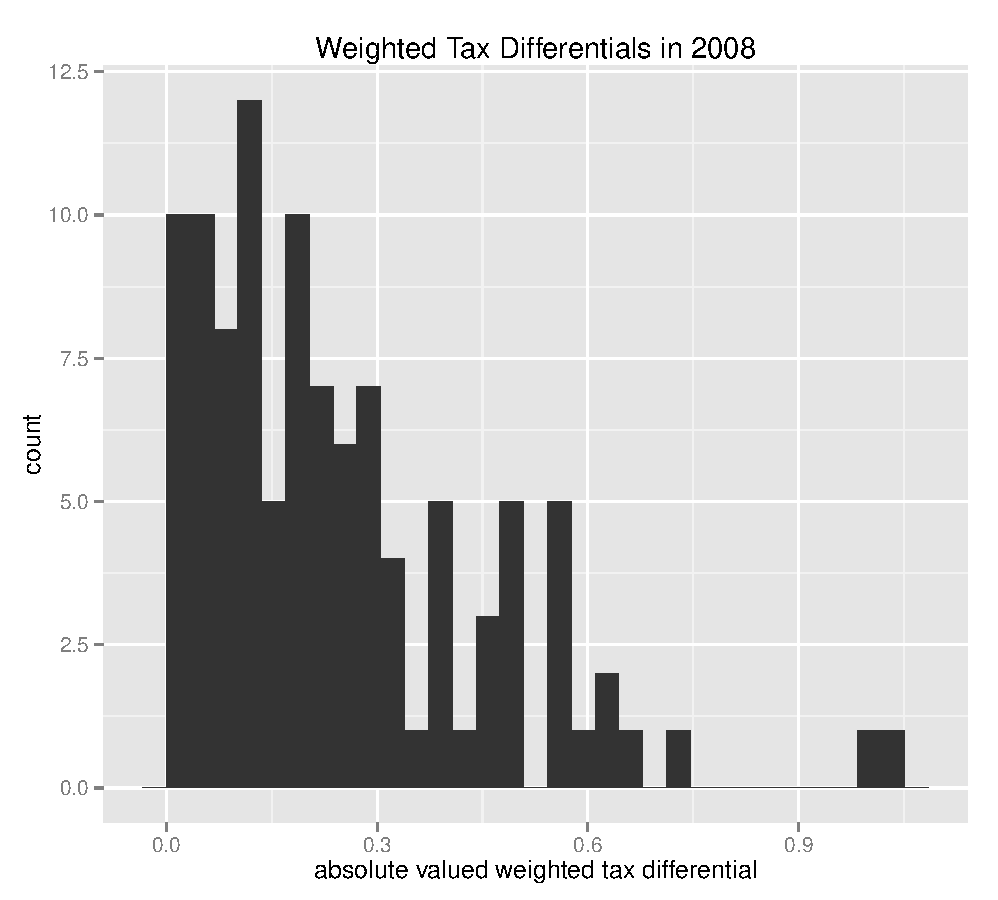
\includegraphics[scale = 0.5]{../../analysis/output/_--_weightedtax.pdf}
\end{figure}
\end{frame}

\begin{frame}
\frametitle{Some Comparisons Pt II}

% Table created by stargazer v.5.2 by Marek Hlavac, Harvard University. E-mail: hlavac at fas.harvard.edu
% Date and time: Mon, Feb 15, 2016 - 10:44:31 AM
\begin{table}[!htbp] \centering 
  \caption{Result Comparison for Estimated Firm Enry} 
  \label{taxtable} 
\tiny 
\begin{tabular}{@{\extracolsep{5pt}} ccccccc} 
\\[-1.8ex]\hline 
\hline \\[-1.8ex] 
mean firm entry & preffered side & abs weighted tax & preferred side & same? & sub state & nbr state \\ 
\hline \\[-1.8ex] 
$0.913$ & nbr & $1.018$ & sub & diff & del. & new jersey \\ 
$0.864$ & sub & $0.998$ & sub & same & nh & vermont \\ 
$0.477$ & sub & $0.719$ & sub & same & maine & nh \\ 
$0.033$ & sub & $0.655$ & nbr & diff & nebraska & wyoming \\ 
$0.219$ & nbr & $0.637$ & nbr & same & delaware & pennsylvania \\ 
$0.763$ & sub & $0.636$ & sub & same & montana & north dakota \\ 
$1.146$ & nbr & $0.608$ & nbr & same & delaware & maryland \\ 
$0.297$ & nbr & $0.565$ & nbr & same & idaho & wyoming \\ 
$0.295$ & nbr & $0.558$ & nbr & same & california & oregon \\ 
$1.743$ & sub & $0.555$ & sub & same & colorado & kansas \\ 
\hline \\[-1.8ex] 
\end{tabular}
\end{table} 

\end{frame}

\begin{frame}
\subsection{Sensitivity Tests}
\frametitle{Sensitivity Tests pt I}

% Table created by stargazer v.5.2 by Marek Hlavac, Harvard University. E-mail: hlavac at fas.harvard.edu
% Date and time: Mon, Feb 15, 2016 - 10:39:15 AM
\begin{table}[!htbp] \centering 
  \caption{Urban to Rural Estimates} 
  \label{--metro} 
  \small 
   {\tiny\renewcommand{\arraystretch}{}
\resizebox{!}{.35\paperheight}{%
\begin{tabular}{@{\extracolsep{5pt}}lcccc} 
\\[-1.8ex]\hline 
\hline \\[-1.8ex] 
 & \multicolumn{4}{c}{\textit{Dependent variable:}} \\ 
\cline{2-5} 
\\[-1.8ex] & \multicolumn{4}{c}{births ratio} \\ 
 & In a MSA & Same MSA & Jointly Urban & Jointly Rural \\ 
\\[-1.8ex] & (1) & (2) & (3) & (4)\\ 
\hline \\[-1.8ex] 
 Property Tax Difference & $-$0.339 & $-$0.153 & $-$0.205 & $-$0.390$^{**}$ \\ 
  & (0.418) & (0.614) & (0.215) & (0.174) \\ 
  Income Tax Difference & $-$0.183$^{***}$ & $-$0.309$^{***}$ & $-$0.124$^{***}$ & $-$0.041 \\ 
  & (0.068) & (0.097) & (0.042) & (0.039) \\ 
  Capital Gains Tax Difference & 0.117$^{*}$ & 0.228$^{***}$ & 0.074$^{*}$ & $-$0.019 \\ 
  & (0.063) & (0.077) & (0.039) & (0.026) \\ 
  Sales Tax Difference & $-$0.132 & $-$0.253$^{***}$ & $-$0.125$^{***}$ & $-$0.069 \\ 
  & (0.086) & (0.086) & (0.048) & (0.053) \\ 
  Corp Tax Difference & 0.020 & 0.031 & $-$0.037 & 0.058$^{**}$ \\ 
  & (0.048) & (0.073) & (0.028) & (0.026) \\ 
  Workers Comp Tax Difference & 0.425$^{**}$ & 0.438 & 0.149 & $-$0.109 \\ 
  & (0.182) & (0.293) & (0.131) & (0.163) \\ 
  Unemp. Tax Difference & 0.098$^{*}$ & 0.084 & 0.031 & $-$0.070 \\ 
  & (0.060) & (0.062) & (0.048) & (0.054) \\ 
  Educ Spending Per Cap Diff & $-$0.001 & $-$0.0004 & $-$0.0001 & $-$0.001$^{*}$ \\ 
  & (0.001) & (0.001) & (0.0004) & (0.0004) \\ 
  Highway Spending Per Cap Diff & $-$0.002$^{*}$ & $-$0.001 & $-$0.00002 & 0.001$^{**}$ \\ 
  & (0.001) & (0.001) & (0.001) & (0.001) \\ 
  Welfare Spending Per Cap Diff & 0.0001 & $-$0.0001 & 0.0002 & 0.001$^{*}$ \\ 
  & (0.001) & (0.001) & (0.0003) & (0.0004) \\ 
  Constant & $-$0.248 & $-$0.507$^{*}$ & $-$0.329$^{***}$ & 0.381$^{***}$ \\ 
  & (0.214) & (0.261) & (0.113) & (0.101) \\ 
 \hline \\[-1.8ex] 
Observations & 2,223 & 1,383 & 8,180 & 4,935 \\ 
R$^{2}$ & 0.117 & 0.168 & 0.050 & 0.089 \\ 
\hline 
\hline \\[-1.8ex] 
\textit{Note:}  & \multicolumn{4}{r}{$^{*}$p$<$0.1; $^{**}$p$<$0.05; $^{***}$p$<$0.01} \\ 
 & \multicolumn{4}{l}{All models are estimated with Ordinary Least Squares} \\ 
 & \multicolumn{4}{l}{and clustered standard errors at the state-pair level.} \\ 
\end{tabular}}}
\end{table} 
\end{frame}

\begin{frame}
Similarly estimated models...
\begin{itemize}
\item ...for different two-digit NAICS industry codes
\item ...for each year in our sample
\begin{itemize}
\item Sales and property taxes remain negative and significant over all time periods. Income taxes start negative but insignificant, and become more negative and significant as time went on
\end{itemize}
\item ...for differerent match lengths
\begin{itemize}
\item We expected the impacts of taxes to go away as we matched counties further away from the border, as location specific terms would be a bigger driver of firm entry decisions
\item all our tax variables become insignificant in these models
\end{itemize}
\end{itemize}
\end{frame}

\begin{frame}
\section{Conclusion}
\frametitle{Conclusion}
Going back to our original two research questions, we see that:
\begin{itemize}
\item Property, sales, and income taxes across most specifications besides for our interaction term regressions. 
\item Property tax rates have a relatively high elasticity, where a 1\% increase in relative property tax rates corresponds to a 0.49\% decrease in relative firm start up rates. A 1\% increase in relative sales and income tax rates correspond to a 0.08\% decrease in relative firm start up rates.
\item Government expenditures on infrastructure, welfare, and education does not seem to impact firm start up. rates.

\end{itemize}
\end{frame}

\begin{frame}
\begin{centering}
\huge{Thank you for your time!}
\end{centering}
\end{frame}
\end{document}